\documentclass[a4paper]{report}
\usepackage{unifrrr}
\usepackage{graphicx}
\usepackage[latin1]{inputenc}
\usepackage{float}
\usepackage[colorlinks=false, pdfborder={0 0 0}]{hyperref}
\usepackage{verbatim}
\usepackage{hyperref}
\usepackage{cite}
\usepackage{bibgerm}
\usepackage[english]{babel}
\usepackage{listings}
\usepackage{color}
\usepackage{appendix}
\usepackage{minitoc}
\definecolor{javared}{rgb}{0.6,0,0} % for strings
\definecolor{javagreen}{rgb}{0.25,0.5,0.35} % comments
\definecolor{javapurple}{rgb}{0.5,0,0.35} % keywords
\definecolor{javadocblue}{rgb}{0.25,0.35,0.75} % javadoc


\lstset{language=Java,
basicstyle=\ttfamily\footnotesize,
keywordstyle=\color{javapurple}\bfseries,
stringstyle=\color{javared},
commentstyle=\color{javagreen},
morecomment=[s][\color{javadocblue}]{/**}{*/},
numbers=left,
numberstyle=\tiny\color{black},
stepnumber=1,
numbersep=10pt,
tabsize=4,
showspaces=false,
showstringspaces=false,
captionpos=b}

\begingroup
    \catcode `\@ = 11
    \catcode `\~ = 13
    \catcode `\% = 12
    \protected\long\gdef\cmt@remove#1%~{\endgroup}
    \ifdefined~
        \global\let\cmt@old~
    \else
        \global\let\cmt@old\relax
    \fi
    \protected\gdef~{\begingroup\catcode`%=12
        \futurelet\next\cmt@}
    \protected\gdef\cmt@
      {\ifx%\next
           \expandafter\cmt@remove
       \else
           \endgroup\expandafter\cmt@old
       \fi}
\endgroup


\setcounter{secnumdepth}{4}
\setcounter{tocdepth}{4}

%--------------------------------------------------------------------


%The body of the LaTeX file
\begin{document}  



%Including of the title page. See titlepage.tex file
%Starting the title page. A \begin command always ends with a \end command
\begin{titlepage} 
	%Center all the following stuff
	\begin{center}
		
		%Include the unifr.jpg file from ./images. \\ is a line break
		
\includegraphics[scale=2]{images/unifr.jpg}\\
		
		%Do a vertical space of 0.5 cm
		\vspace{0.5cm}
		
		
	
		\vspace{2cm}
		
		\begin{Large}
		Master Thesis\\
		\end{Large}
		
		\vspace{2cm}
		
		%Start a huge font
		\begin{huge}
			%Sans serif
			{\sf \bf Crowdsourced Product Descriptions and Price Estimations}
		\end{huge}
		
				
		\vspace{2cm}
		
		 Steve Aschwanden\\
		 Dammstrasse 4\\
		 CH-2540 Grenchen\\
		 steve.aschwanden@students.unibe.ch\\
		 05-480-686\\
		
		\vspace{1.5cm}
		
		{\bf Supervisor}\\
		Dr. Gianluca Demartini\\
		C302, Bd de P�rolles 90\\
		CH-1700 Fribourg\\
		demartini@exascale.info\\
		\vspace{2.5cm}
		
		
		Grenchen, \today\\
		
				
	\end{center}
\end{titlepage}


\pagenumbering{arabic}
\pagestyle{plain}
\newpage

\chapter*{Declaration}
\thispagestyle{empty}

\vspace{0.2in}
I declare that this written submission represents my ideas in my own words and where others' ideas or words have been included, I have adequately cited and referenced the original sources. I also declare that I have adhered to all the principles of academic honesty and integrity and have not misrepresented or fabricated or falsified any \mbox{idea/data/fact/source} in my submission. I understand that any violation of the above will be cause for disciplinary action by the Institute and can also evoke penal action from the sources which have thus not been properly cited or from whom proper permission has not been taken when needed.
\vspace{1in}
%\begin{table*}[hb]
\begin{center}
\begin{tabular*}{\textwidth}{@{\extracolsep{\fill}} lr }
\vspace{0.5in}
& Steve Aschwanden, 05-480-686\\
Grenchen; \today: & \hrulefill \\
& (Signature)\\
\end{tabular*}
\end{center}
\chapter*{Acknowledgements}
\thispagestyle{empty}
I like to acknowledge ...
\clearpage
\chapter*{Abstract}
\thispagestyle{empty}
The creation of auctions for the online marketplace eBay is time consuming and repetitive. The first step for selling an item is taking pictures of it. To complete the auction, the user has to provide a title, description, category and other predefined parameters. One of the most important step is the definition of a starting price.\\\\
Crowdsourcing is used to generate the required information for a complete auction based on several images. The complex task is split into multiple subtasks. The thesis presents a pure and a hybrid crowdsourcing approach. Different experiments were made to investigate the behaviour of the crowd.\\\\
A promised commission for successful auctions has the biggest influence to the quality of the workers. A majority favours the results of this experiment over the descriptions of the corresponding real online auction. The workers did the most accurate price predictions if the actual market price of the items is provided.\\\\  
The results of the executed experiments show the potential of the crowd. If all the strength of the single variations will be combined and the task design is improved slightly then the generated contents can be used to create real auctions on eBay in the future.
\clearpage


\dominitoc
\tableofcontents
\newpage

\listoffigures

\listoftables

\lstlistoflistings

\chapter{Introduction}
eBay Inc.\footnote{http://www.ebay.com} is one of the world's largest online marketplaces and reported 128 million active users worldwide during the last quarter of the year 2013. Online auction platforms make consumer-to-consumer transactions possible. The seller can present articles by uploading pictures and describing them. The creation of an auction is time consuming and needs a lot of investigations. Searching for descriptions on the internet or finding a selling price for the same or similar article, for example. In 2005, Jeff Howe and Mark Robinson created a term called 'Crowdsourcing' which is a combination of the words crowd and outsourcing. The idea behind the term is to outsource different tasks, which are difficult to solve by machines, to the crowd. To reduce the costs of collecting information for an article to sell on an auction platform, tasks will be created and outsourced to the crowd. Amazon Mechanical Turk\footnote{http://www.mturk.com}, short MTurk, is a crowdsourcing marketplace which enables requesters to publish human intelligence tasks (HITs). The workers can solve these tasks and earn money for good work.

\section{Statement of the problem}
The first step of creating an online auction is mostly to take pictures of the corresponding item. This help the buyers to get information about the state and quality of the article. After that the item needs a short and clear description, some properties (category, state) and a starting offer. If the seller wants to create a lot of different auctions, the whole procedure is time consuming and boring. A price estimation of an article can be difficult, because the background knowledge is missing and other auctions to compare aren't available at any time. Machines aren't able to solve all these steps by them self, because the spectrum of the articles is huge and image processing methods aren't capable to classify them all correctly. To get all the needed parts of an online auction, a human powered approach is necessary. Crowdsourcing platforms provide the possibility to solve tasks, which are difficult to handle for a computer.

\section{Existing research}
tbd

\section{Goals and objectives}
The thesis has the following goals and their corresponding objectives:
\begin{itemize}
	\item \textbf{Collect auction item properties by the crowd}
	\begin{itemize}
		\item Analyse the composition of an auction item on eBay and select the parts which can be crowdsourced
		\item Form a ground truth including different auctions created by real online auction platform users by using the eBay API
		\item Study literature which covers similar crowdsourcing problems
		\item Design and publish tasks on Amazon Mechanical Turk to gather data from the crowd
		\item Evaluate the quality of the generated content
	\end{itemize}
	\item \textbf{Try to improve the initial solution by implementing a hybrid approach}
	\begin{itemize}
		\item Search for image processing or machine learning methods which can simplify and/or support a human intelligence task
		\item Implement the methods and adapt the design of the tasks
		\item Publish the new tasks on the same crowdsourcing platform
		\item Evaluate the results and compare them to the first solution 
	\end{itemize}
\end{itemize}

If the main goals of the thesis are fulfilled, some \textit{optional} goals can be covered by the thesis:
\begin{itemize}
	\item \textbf{Implement a web application which combines the created subtasks to a complete workflow}
	\begin{itemize}
		\item Find a web application framework which provide an API in the same programming language as the Amazon Mechanical Turk API
		\item Create a workflow which put all the subtasks together to an overall solution
		\item The user can manage the items (upload pictures to create new items, edit and remove items) and directly create an online auction
	\end{itemize}
\end{itemize}

\section{Organization}
The thesis is splited into several chapters:
\begin{itemize}
	\item eBay online marketplace
	\item Crowdsourcing
	\item Evaluation
	\item Conclusion
\end{itemize}

\chapter{eBay online marketplace}
\minitoc
\section{History}
eBay was founded 1995 in San Jose (CA) as AuctionWeb by Pierre Omidyar. One year later, eBay bought a third-party licence from Electronic Travel Auction to sell plane tickets and other travelling stuff. During the year 1996, over 200'000 auctions were available on the website. At the beginning of 1997 the number of auctions exploded (about 2 million articles). In the same year the company get their well-known name eBay and received 6.7 million dollar from the venture capital firm Benchmark Capital. The company went public on the stock exchange on September 21, 1998 and the share price increased from 18 to 53.5 dollar on the first day of trading. Four years later the growth continues and eBay bought the online money transfer service PayPal. eBay expanded worldwide in early 2008, had hundred millions of registered users and 15'000 employees. Today, the firm is one of the world's largest online marketplaces. During the fourth quarter of the year 2013 about 128 million active users were reported. A cell phone was sold every 4 seconds, a pair of shoes every 2 seconds and a Ford Mustang every 55 minutes.

\section{Auction item composition}
Every eBay user has the possibility to create auctions for different kind of items. To present the article, the seller has to provide accurate information about it. The standard eBay auction consists of the following fields:
\begin{itemize}
	\item \textbf{Title} The title of the item is limited to 80 characters. The sellers should use descriptive keywords to clearly and accurately convey what they are selling
	\item \textbf{Description} The description is the opportunity to provide the buyers with more information about the item
	\item \textbf{Category} An item can have multiple predefined categories. eBay provides a list of categories which the seller can select
	\item \textbf{Condition} The condition of the item is dependent on the selected category. eBay provides different condition schemas. For clothing items the seller can select between 'New with tags', 'New without tags', 'New with defects' or 'Pre-owned'. For other categories like books, other condition values are present: 'Brand new', 'Like new', 'Very good', 'Good', 'Acceptable'
	\item \textbf{Pictures} To visualise the item the auction creator can upload up to twelve pictures. The first image is important, because it appears next to the item's title in the search result. The pictures will be stored for 90 days on the eBay servers.
	\item \textbf{Shipping costs} The seller has to tell the future buyers how much shipping will cost. There are three possibilities:
	\begin{itemize}
		\item Free shipping
		\item Flat shipping, same cost to all buyers
		\item Shipping rate tables, eBay calculates the cost for every individual buyer dependent on the location
	\end{itemize}
	\item \textbf{Duration} An auction can have a duration of 1, 3, 5, 7 or 10 days. If the item has a fixed price, the auction is finished if a buyer is willing to pay this price.
	\item \textbf{Pricing} The seller can select a starting price and then the bidding will start at this price. A 'But it now' option is also available. The buyer can skip the bidding process.
	\item \textbf{Payment} The seller has to select the desired paying method like 'PayPal' or 'Payment upon pickup'
\end{itemize}

\section{APIs}
eBay provides multiple APIs for developing third party applications. This allows developers to search for auctions or create listings over the XML format. Three main interfaces are available:
\begin{figure}[h!]
\centering
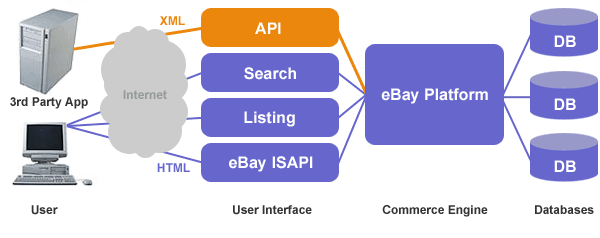
\includegraphics[scale=0.5]{images/api-flow.png}
\caption{eBay API overview}
\label{ebayAPI}
\end{figure}

\subsection{Trading API}
Developers use the Trading API to build applications such as selling and post-sales management applications, manage user information, and initiate the item purchase flow on eBay. The API is available in .NET, Java, PHP and Python.

\subsection{Shopping API}
The Shopping API provides a search engine for user information, popular items and reviews. The API is available in PHP and Python. Example calls for this API are:
\begin{itemize}
	\item \textit{findProducts()}: Search for products by keywords or ProductId
	\item \textit{GetSingleItem()}: Buyer specific view of an item
	\item \textit{GetUserProfile()}: Get the user profile and feedback information
\end{itemize}

\subsection{Finding API}
The Finding API provides access to the next generation search capabilities on the eBay platform. The developer can search and browse for items based on keyword queries, categories or an image. The API is available in .NET, Java and Python. Example calls for this API are:
\begin{itemize}
	\item \textit{findCompletedItems()}: Find the items which are listened as completed or no longer available on eBay
	\item \textit{findItemsByCategory()}: Find items in a specific category
	\item \textit{findItemsByImage()}: Find items which have a high similarity to a given image
\end{itemize}

\subsection{Example}
The following listing in Python illustrate the functionality of the Finding API. The developer has to register to the eBay developers program first. After that, a application ID can be created. This is necessary to get access to the eBay databases. A functioning Python environment and the additional eBay Python SDK are requirements to successfully execute the example
\lstset{language=Python,caption={eBay Finding API example},label=findingapi_example}
\begin{lstlisting}
from ebaysdk.finding import Connection as Finding
from ebaysdk.exception import ConnectionError
import json

try:
    api = Finding(appid='Universi-3c25-4b4e-b3e6-8c2568808b12')
    api.execute('findCompletedItems', {
        'keywords': 'ford mustang',
        'itemFilter': [
            {'name': 'ListingType',
             'value': 'Auction'},
            {'name': 'Currency',
             'value': 'USD'},                
            {'name': 'SoldItemsOnly',
             'value': 'true'},                 
        ],        
        'sortOrder': 'StartTimeNewest',
        })
    response = json.loads(api.response_json())
    
    print response['searchResult']['item'][0]
    
except ConnectionError as e:
    raise e  
\end{lstlisting}
The initialisation of the application is done on line 6. A correct application ID is required. Then the API call \textit{findCompletedItems()} is executed with some keywords and filter options. Only the newest auctions with at least one bidder and a payment in US dollar will be returned. The function \textit{response\_json()} (on line 19) returns the first 100 items by default. At the end, the first result will be printed to the console. Here is a shorter simplified version with the most important fields of the output:
\begin{table}[h!]
	\begin{center}
	\begin{tabular}{| l | l |}
		\hline
		\textbf{Name} & \textbf{Value} \\
		\hline
		itemId & 281273507096 \\
		\hline
		title & 2014 Hot Wheels Super Treasure Hunt 71 Mustang Mach 1 \\
		\hline
		categoryName & Diecast-Modern Manufacture \\
		\hline
		shippingType & Calculated \\
		\hline
		currentPrice & 18.5 USD \\
		\hline
		bidCount & 1 \\
		\hline
		paymentMethod & PayPal \\
		\hline
		conditionDisplayName & New \\
		\hline
		startTime & 2014-02-25T04:32:17.000Z \\
		\hline
		endTime & 2014-02-25T05:27:14.000Z \\
		\hline
	\end{tabular}
	\end{center}
	\caption{eBay Finding API example output}
\end{table}


\clearpage

\selectlanguage{english}
\bibliographystyle{bib/custom}
\bibliography{bib/references}
\newpage
\begin{appendices}
\chapter{Some Appendix}


\section{README}
\lstset{caption={}}
\begin{lstlisting}
Fuzzily classify twitter messages using storm and store to cassandra
===


Setup Cassandra (on ubuntu):
---
1. Make sure oracle JDK is installed (1.6+): https://help.ubuntu.com/community/Java#Oracle_Java_7
2. Add the DataStax repository key to your aptitude trusted keys.
> $ curl -L http://debian.datastax.com/debian/repo_key | sudo apt-key add -
3. Install Cassandra:
> sudo apt-get update && sudo apt-get install cassandra
4. Create keyspace and tables:
> cqlsh
> run commands from src/main/resources/createDatabase.txt

Build Runnable jar
---
1. Open a terminal window, navigate to pom.xml directory (project root)
2. Execute the following command:
> mvn clean compile assembly:single
3. In target/, a runnable jar tsfc.jar is created

Run Program
---
> java -jar tsfc.jar <<comma separated list of topics to watch (without whitespace)>>
\end{lstlisting}

\end{appendices}

\end{document}
